\section{Miscellaneous Notes}
% the text width in a normal line is 11.80737cm
% To make a TODO note, start a comment with two or more consecutive capital letters.

% Figures are in the gfx folder. They should not have dots in the names
% since that interferes with the crossref function. They should be named
% something like '01-intro.png' where the first two digits are the 
% chapter number and then some simple description of the figure.

% Potential arrangement (for 2nd ed???): 
%		3 Background chapters
%		8 Chapters about ``Traditional'' procedures
%		4 Chapters about Business Analytics, datamining, etc.

% TODO
% add photo to start of each chapter
 

% TODO: Status
% FIXME

%Background
% 01 Intro: Glossary and Biblio checked 
% 02 Foundations: Glossary and Biblio checked
% 03 Ethics: Glossary and Biblio checked
% 04 Design: Glossary and Biblio checked

% Quantitative
% 05 Measuring: Glossary and Biblio checked
% 06 Data: 1st Draft
% 07 Sampling: 1st Draft (illustrations done)
% 08 Surveys: Pre-draft
% 09 Interviews: Pre-draft
% 10 Experimental: Pre-draft

% Qualitative
% 11 Field: Pre-draft
% 12 Unobtrusive: Pre-draft
% 13 Interpretive: Pre-draft

% Mixed Methods
% 14 Mixed: Empty

% Reporting
% 15 Presenting: Pre-draft

%************************************************************
\section{acronyms and glossary}
% all acronymns and glossary entries are defined in
% AcroGloss.tex. I have some information in that document
% about how to format entries.
% To compile the glossary:
% 1. Build the document
% 2. Tools -> Glossary (F9) % to build the glossary entries
% 3. Build the document again

% To use an acronym or glossary term in the text (they are the same):
%***************************************************************
\gls{code} % Where ``code'' is the code I specify in the glossary entry
\glspl{code} % For the plural (note: forms a simple ``s'' plural)
% for more complex plurals, create an alternate form in AcroGloss
\Gls{code} % Capitalize the first letter
\Glspl{code} % Capitalize the first letter, make the word plural


%******************************************************
\section{3-Line Equation}
%******************************************************
\begin{align}
	\label{03:eq:identity_example}
	1101_2 &= 123 \\
	\nonumber
	&= 123 \\
	\nonumber
	&= 123
\end{align}


\section{Solving an Equation Step-by-step}
\begin{align}
	\label{04:soln:solving_equation_one}
	AB+BC(B+C) && \text{Original Expression} \\
	\nonumber
	AB+BBC+BCC && \text{Distribute BC} \\
	\nonumber
	AB+BC+BC && \text{Idempotence: BB=B and CC=C} \\
	\nonumber
	AB+BC && \text{Idempotence: BC+BC=BC} \\
	\nonumber
	B(A+C) && \text{Factor} \\
\end{align}

%**************************************************************************
\section{Margin Paragraph} 
%**************************************************************************
% Use to create a sidebar paragraph out in the margin
\marginpar{Whatever.}

%**************************************************************************
\section{Footnote Without Marker} 
%**************************************************************************
% Use to create a footnote without a numbering marker
\blfootnote{Whatever.}

%***************************************************************************
\section{Text Box}
%***************************************************************************
% Creates a nice boxed text with a title and main section
\begin{tcolorbox}[colback=blue!5!white,colframe=blue!75!black]
	% Upper half of box: my "title" area
	\textcolor{blue}{\textbf{Interesing Note}}
	% Lower half of the box: the content
	\tcblower
	Whatever.
\end{tcolorbox}

%***************************************************************************
\section{Objectives Box}
% Relies on ``objbox'' in config file
%***************************************************************************
\begin{center}
	\begin{objbox}{Objectives}
		\begin{itemize}
			\setlength{\itemsep}{0pt}
			\setlength{\parskip}{0pt}
			\setlength{\parsep}{0pt}
		
			\item x1.
			\item x2.
			\item x3.
		\end{itemize}
	\end{objbox}
\end{center}


%***************************************************************************
\section{Text Table}
%***************************************************************************
% the p values set column width and force word wrap, left align text
% the p values should total 0.95, the width of the table
\begin{table}[H]
	\centering
	\definecolor{ltgray}{gray}{0.95} % this is a light gray
	\rowcolors{1}{}{ltgray} % zebra striping background
	\begin{tabularx}{0.95\linewidth}{p{0.15\linewidth}p{0.40\linewidth}p{0.40\linewidth}}
		\toprule
		\textbf{X} & \textbf{Y} & \textbf{Z} \\
		\midrule
		a & b & c \\
		a & b & c \\
		a & b & c \\
		a \newline b & b & c \\ % line break in cell
		\midrule
		\multicolumn{3}{p{0.95\linewidth}}{Note: def.} \\	
		\bottomrule
	\end{tabularx}
	\caption{My great table.}
	\label{tab06.01}
\end{table}

%*************************************
% Tabulary will automatically adjust the column widths and word wrap
%*************************************

\begin{tabulary}{\linewidth}{LCCCC}
	\hline
	\multicolumn{5}{l}{\textbf{Do you support these propositions?}} \\
	\hline
	Prop & Strongly Support & Support & Do Not Support & Strongly Do Not Support  \\ 
	\hline
	100 & $\bigcirc$ & $\bigcirc$ & $\bigcirc$ & $\bigcirc$ \\ 
	115 & $\bigcirc$ & $\bigcirc$ & $\bigcirc$ & $\bigcirc$ \\ 
	220 & $\bigcirc$ & $\bigcirc$ & $\bigcirc$ & $\bigcirc$ \\ 
	\hline
\end{tabulary} 

\vspace{.15in}


%***************************************************************************
\section{ToDo}
%***************************************************************************
% Create a ToDo note in the text. This also creates a new clickable TODO
% section in the ``structure'' box on the left side of the page.
%TODO This is a todo note.

%***************************************************************************
\section{Code Snip}
%***************************************************************************
\lstset{ %
  caption={caption},
  label=SL:lst:listing01,
  numbers=left,
  language=Verilog
}
\begin{lstlisting}
  Code here
\end{lstlisting}

%***************************************************************************
\section{Introductory Figure}
%**************************************************************************
% Use this for figures at the top of each chapter

\section{first section head}

\begin{wrapfigure}{r}{0.4\textwidth}
	\label{fig01.01} 
	\centering
	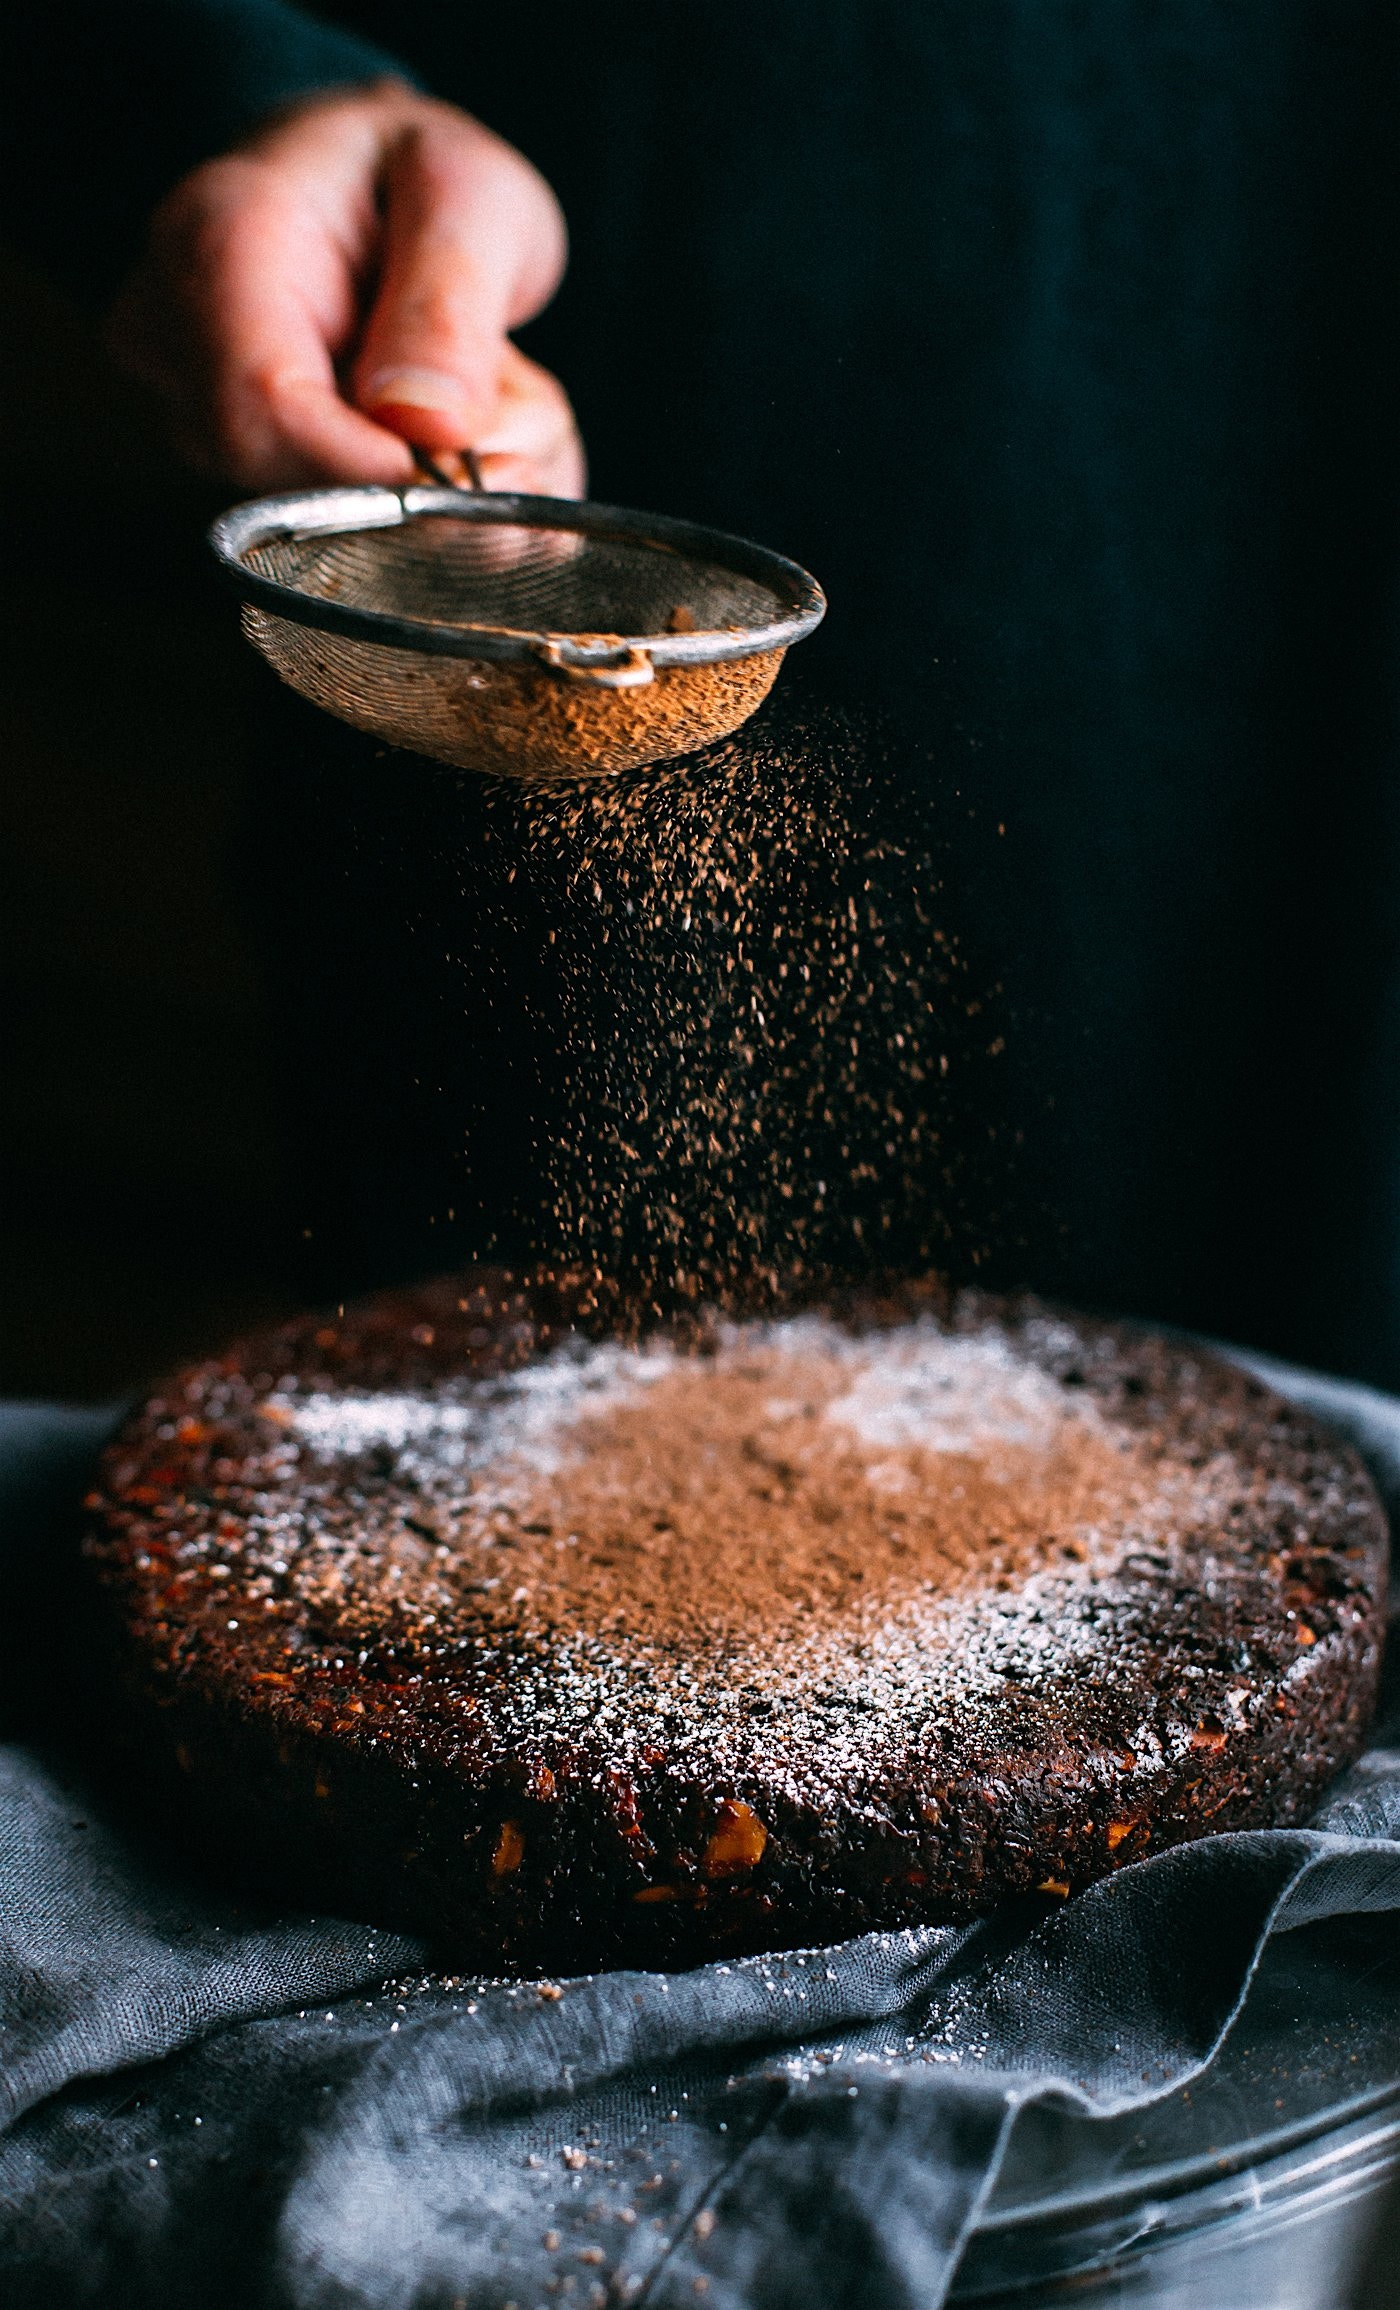
\includegraphics[width=0.4\textwidth]{gfx/05-cake} 
\end{wrapfigure}

First paragraph.\blfootnote{Photo by lindsay Cotter on Unsplash}

%***************************************************************************
\section{Wrap Figure}
%**************************************************************************
\begin{wrapfigure}{O}{0.2\textwidth}
	\caption{} % No text, wraps badly in very narrow space (does print fig number)
	\label{fig01.01} 
	\centering
	
\includegraphics[width=0.2\textwidth]{gfx/99-placeholder} 
\end{wrapfigure}

%***************************************************************************
\section{Regular Figure}
%**************************************************************************
\begin{figure}[H]
	\centering
	
\includegraphics[width=\maxwidth{.95\linewidth}]{gfx/99-placeholder}
	\caption{Caption}
	\label{fig01.01}
\end{figure}

%***************************************************************************
\section{Style Guide}
%**************************************************************************

For menu selections:
Click \textsc{\fbox{Analyze $ \rightarrow $ Descriptive Statistics $ \rightarrow $ Frequencies}}

Labels should be a chapter, colon, verbal desc (all lc with underscores): \label{03:title}
For figures, label should be chapter, colon, ``fig'' and number: \label{03:fig01}

Dates do not include an apostrophe: In the 1960s this happened...

Wrap all numbers in an in-line math block: $ 123 $

